%!TEX root = ../main.tex

\chapter{Numerische Experimente} % (fold)
\label{cha:numerische_experimente}

% section grundlagen_zum_galerkin_verfahren (end)

\section{Erste Versuche mit Galerkin-Projektion} % (fold)
\label{sec:erste_versuche_mit_galerkin_projektion}

Wir beschränken uns erneut auf den eindimensionalen Fall und wählen $T = 1$, also $I = [0, 1]$ und $\Omega = [0 ,1]$.
Um eine Approximation für das Variationsproblem \eqref{eq:varprob} mit fest gewähltem $\omega \in L_{\infty}(\Omega)$ zu bestimmen, verwenden wir die Galerkin-Projektion.

Dazu definieren wir endlichdimensionale Unterräume $\mathcal X_{\mathcal N} \subset \mathcal X$ und $\mathcal Y_{\mathcal M} \subset \mathcal Y$, wobei $\dim(\mathcal X_{\mathcal N}) = \mathcal N$ respektive $\dim(\mathcal Y_{\mathcal M}) = \mathcal M$ sei.
Der Einfachheit halber fordern wir zunächst $\mathcal N = \mathcal M$.
Das nun zu lösende Problem lautet damit

\begin{Problem}
    Gegeben ein $g \in L_{2}(I; V')$ und ein $u_{0} \in H$. Finde ein $u \in \mathcal X_{\mathcal N}$ mit
    \begin{equation}
        \label{eq:varprob_3}
        b(u, v) = f(v) \quad \text{für alle}~v \in \mathcal Y_{\mathcal M}.
    \end{equation}
\end{Problem}

Wie wählt man nun die endlichdimensionalen Unterräume $\mathcal X_{\mathcal N}$ und $\mathcal Y_{\mathcal M}$?

\paragraph{Erster Versuch} % (fold)
\label{par:erster_versuch}

Da wir es mit homogenen Randbedingungen zu tun haben, ist es naheliegend, Sinusfunktionen $\sin(\pi j x)$, $j \geq 1$, als Basisfunktionen für die Raum-Koordinate zu verwenden.
Für die Zeitkoordinate wählen wir orthogonale Polynome, konkret auf den Intervall $I = [0, 1]$ verschobene Legendre-Polynome $L_{k}$, $k \geq 0$.

Die Idee hinter der Wahl der orthogonalen Polynome, und auch der Sinusfunktionen, ist, dass diese bezüglich der $L_{2}$-Norm jeweils ein orthogonales System bilden, wodurch für die Galerkin-Projektion aufzustellende Steifigkeitsmatrix $\mat B$ dünn besetzt ist.

Da wir $\mathcal N = \mathcal M$ erreichen wollen, wählen wir $M, Q \in \mathbb{N}$ und setzen
\begin{equation}
    \mathcal X_{\mathcal N} = \spn\Set{ \sin(\pi j x) L_{k}(t) \given j = 1 \dots M, k = 0 \dots Q }
\end{equation}
und
\begin{equation}
    \mathcal Y_{\mathcal M} = \spn\Set{ (\sin(\pi l x) L_{m}(t), \sin(\pi n x)) \given l, n = 1 \dots M, m = 0 \dots Q - 1 }.
\end{equation}
Damit ergibt sich $\mathcal N = \dim(\mathcal X_{\mathcal N}) = M (Q + 1)$ und $\mathcal M = \dim(\mathcal Y_{\mathcal M}) = M Q + M = M ( Q + 1 )$, also $\mathcal N = \mathcal M$.

Für die Galerkin-Projektion berechnen wir nun
\begin{equation}
    \mat B_{ij} = b(u_{j}, v_{i}) \quad\text{und}\quad \vec f_{i} = f(v_{i}),
\end{equation}
lösen anschließend das lineare Gleichungssystem
\begin{equation}
    \mat B \vec u = \vec f
\end{equation}
und bestimmen die Lösung $u \in \mathcal X_{\mathcal N}$ als Linearkombination der Ansatzfunktionen von $\mathcal X_{\mathcal N}$ mit den zugehörigen Koeffizienten aus $\vec u$.

Um die Funktionsweise an einem einfachen Beispiel zu überprüfen, wählen wir $w = 1$, $u_{0}(x) = x \sin(\pi x)$ und $g = 0$.
Damit wird die Bilinearform $b(\blank, \blank)$ für $u(t, x) = \sin(\pi j x) L_{k}(t)$ und $v(t,x) = (v_{1}(t,x), v_{2}(t,x)) = (\sin(\pi l x) L_{m}(t), \sin(\pi n x))$ zu
\begin{subequations}
    \begin{align}
    b(u, v)
        &= \int_{I} \skprod{u_{t}(t)}{v_{1}(t)}_{V' \times V} + a(u(t), v_{1}(t)) \diff t + \skprod{u(0)}{v_{2}}_{H}
        \\&= \int_{I} \int_{\Omega} \sin(\pi j x) L_{k}'(t) \sin(\pi l x) L_{m}(t) \diff x \diff t \label{eq:int1}
        \\&\quad  + \int_{I} \int_{\Omega} j l \pi^2 \cos(\pi j x) L_{k}(t) \cos(\pi l x) L_{m}(t) \diff x \diff t  \label{eq:int2}
        \\&\quad + \int_{I} \int_{\Omega} \omega(x) \sin(\pi j x) L_{k}(t) \sin(\pi l x) L_{m}(t) \diff x \diff t  \label{eq:int3}
        \\&\quad + \int_{\Omega} \sin(\pi j x) L_{k}(0) \sin(\pi n x) \diff x  \label{eq:int4}
        % \\&=
    \end{align}
\end{subequations}

Unter Verwendung der Orthogonalität der Legendre-Polynome und der Sinusfunktionen, vgl. \thref{satz:legendre_polynome_orthogonal} respektive \thref{satz:trigonometrische_funktionen_orthogonal}, vereinfachen wir die obigen Integral soweit möglich.
Für das zweite und das vierte Integral erhalten wir so die expliziten Ausdrücke
\begin{equation}
    \int_{I} \int_{\Omega} j l \pi^2 \cos(\pi j x) L_{k}(t) \cos(\pi l x) L_{m}(t) \diff x \diff t
    = \frac{(j \pi)^{2}}{2(2k + 1)} \delta_{j l}  \delta_{k m},
\end{equation}
respektive
\begin{equation}
    \int_{\Omega} \sin(\pi j x) L_{k}(0) \sin(\pi n x) \diff x = (-1)^{k} \frac{1}{2} \delta_{jn}.
\end{equation}
Das erste und das dritte Integral werden zu
\begin{equation}
    \int_{I} \int_{\Omega} \sin(\pi j x) L_{k}'(t) \sin(\pi l x) L_{m}(t) \diff x \diff t
    = \frac{1}{2} \delta_{j l} \int_{I} L_{k}'(t) L_{m}(t) \diff t
\end{equation}
und
\begin{equation}
    \int_{I} \int_{\Omega} \omega(x) \sin(\pi j x) L_{k}(t) \sin(\pi l x) L_{m}(t) \diff x \diff t
    = \frac{1}{2k +1} \delta_{k m} \int_{\Omega} \omega(x) \sin(\pi j x)\sin(\pi l x) \diff x.
\end{equation}

% TODO: Alten Stuff raus!
% \begin{align}
%     &\int_{I} \int_{\Omega} \sin(\pi j x) L_{k}'(t) \sin(\pi l x) L_{m}(t) \diff x \diff t
%     \\&\qquad = \int_{I} L_{k}'(t) L_{m}(t) \diff t \int_{\Omega} \sin(\pi j x) \sin(\pi l x) \diff x
%     \\&\qquad= \frac{1}{2} \delta_{j l} \int_{I} L_{k}'(t) L_{m}(t) \diff t
% \end{align}
% \begin{align}
%     &\int_{I} \int_{\Omega} j l \pi^2 \cos(\pi j x) L_{k}(t) \cos(\pi l x) L_{m}(t) \diff x \diff t
%     \\&\qquad = j l \pi^{2} \int_{I} L_{k}(t) L_{m}(t) \diff t \int_{\Omega} \cos(\pi j x) \cos(\pi l x) \diff x
%     \\&\qquad = \frac{(j \pi)^{2}}{2(2k + 1)} \delta_{j l}  \delta_{k m}
% \end{align}
% \begin{align}
%     &\int_{I} \int_{\Omega} \omega(x) \sin(\pi j x) L_{k}(t) \sin(\pi l x) L_{m}(t) \diff x \diff t
%     \\&\qquad = \int_{I} L_{k}(t) L_{m}(t) \diff t \int_{\Omega} \omega(x) \sin(\pi j x)\sin(\pi l x) \diff x
%     \\&\qquad = \frac{1}{2k +1} \delta_{k m} \int_{\Omega} \omega(x) \sin(\pi j x)\sin(\pi l x) \diff x
% \end{align}

Neben der Steifigkeitsmatrix $\mat B$ benötigen wir auch den Lastvektor $\vec f$, wobei $\vec f_{i} = f(v_{i})$, $i = 1 \dots \mathcal N$.
Konkret wird dies, mit dem gleichen $v \in \mathcal Y_{\mathcal N}$ wie oben, zu
\begin{align}
    f(v)
    &= \int_{I} \skprod{g(t)}{v_{1}(t)}_{V' \times V} \diff t + \skprod{u_{0}}{v_{2}}_{H}
    \\&= \int_{I} \int_{\Omega} g(t, x) \sin(\pi l x) L_{m}(t) \diff x \diff t + \int_{\Omega} u_{0}(x) \sin(\pi n x) \diff x.
\end{align}
Diese beiden Integrale können im Allgemeinen nicht wie die vorherigen direkt ausgewertet werden und müssen mittels numerischer Quadratur approximiert werden.

Sind Steifigkeitsmatrix und Lastvektor bestimmt, dann liefert die Lösung $\vec u$ des linearen Gleichungssystems $\mat B \vec u = \vec f$ einen Koeffizientenvektor, aus dem wir mittels
\begin{equation}
    u_{\mathcal N}(t, x) = \sum_{j = 1}^{M} \sum_{k = 0}^{Q} \vec u_{jk} \sin(\pi j x) L_{k}(t)
\end{equation}
die Näherungslösung $u_{\mathcal N} \in \mathcal X_{\mathcal N}$ des Problems \eqref{eq:varprob_3} erhalten.

% paragraph erster_versuch (end)

% section erste_versuche_mit_galerkin_projektion (end)

\clearpage
\begin{figure}[tb]
    \begin{center}
        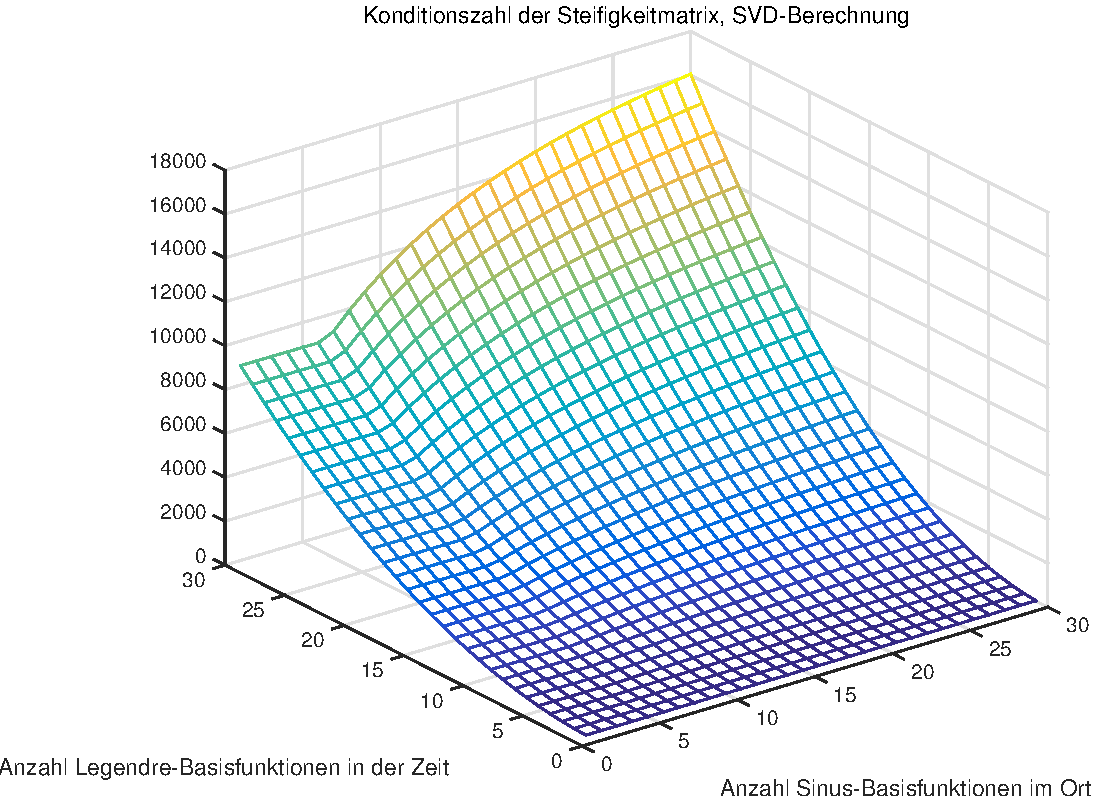
\includegraphics[width=0.9\textwidth]{figures/oned/conds.pdf}
    \end{center}
\end{figure}

\begin{figure}[tb]
    \begin{center}
        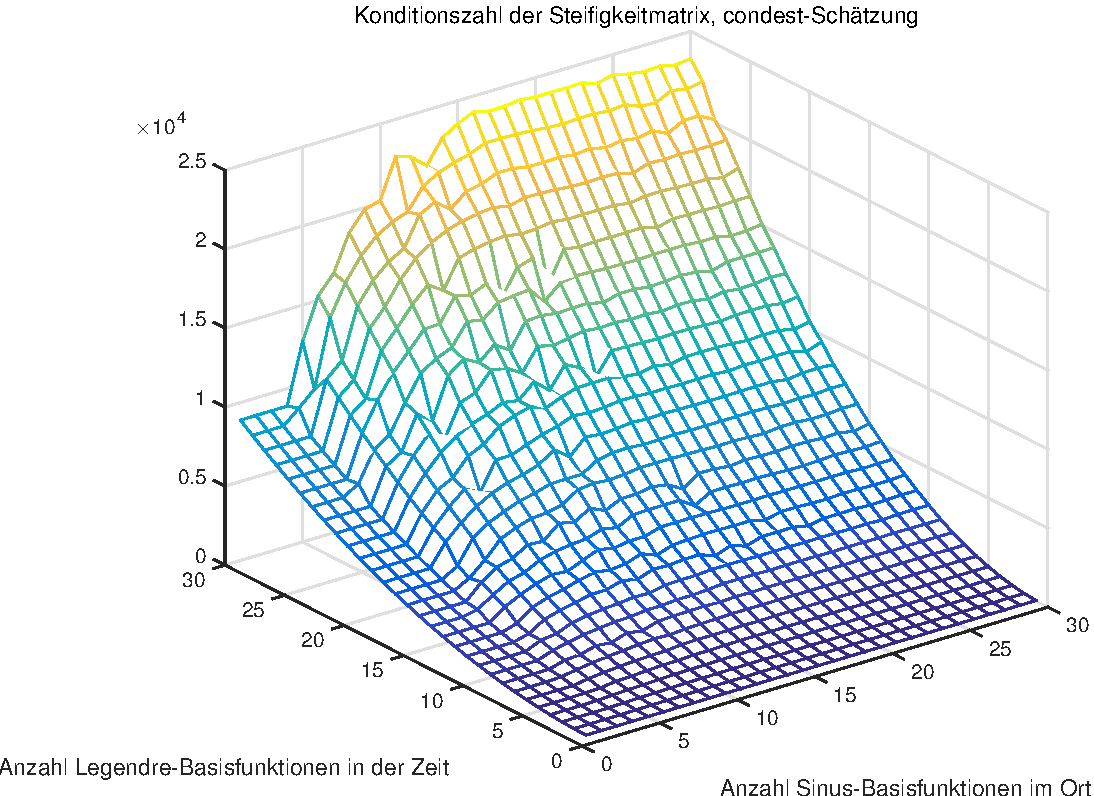
\includegraphics[width=0.9\textwidth]{figures/oned/condest.pdf}
    \end{center}
\end{figure}

\begin{figure}[tb]
    \begin{center}
        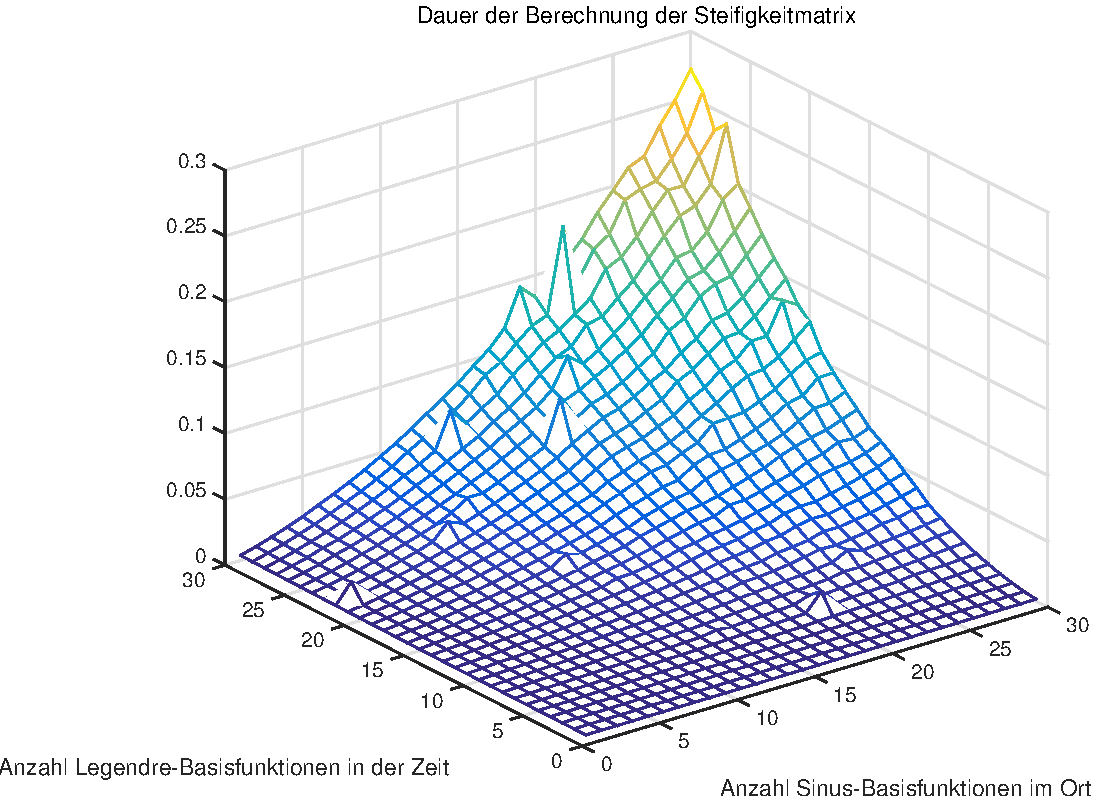
\includegraphics[width=0.9\textwidth]{figures/oned/times.pdf}
    \end{center}
\end{figure}

\begin{figure}[tb]
    \begin{center}
        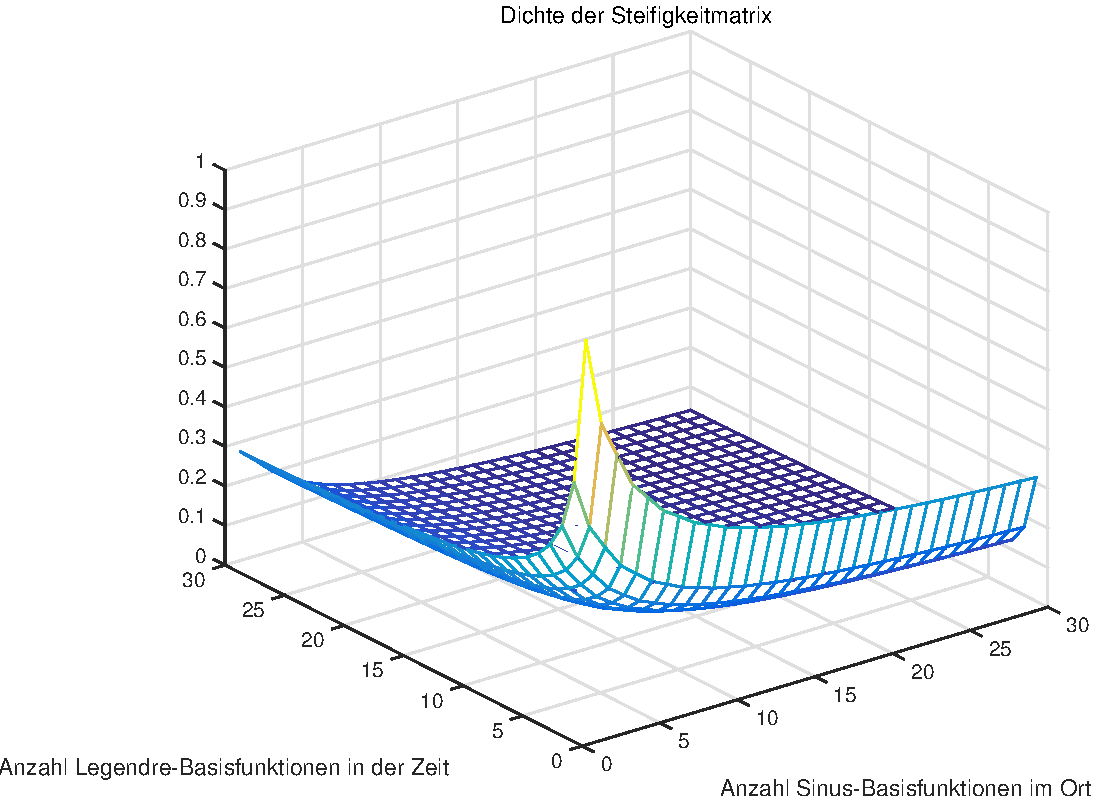
\includegraphics[width=0.9\textwidth]{figures/oned/density.pdf}
    \end{center}
\end{figure}

\clearpage
\begin{landscape}
\thispagestyle{empty}
\begin{table}[tb]
    % \begin{center}
        \hspace{-7em}
        \begin{tabular}{|l|c|c|c|c|c|c|c|c|c|c|c|c|c|c|} \hline
           & 1 & 2 & 3 & 4 & 5 & 6 & 7 & 8 & 9 & 10 & 15 & 20 & 25 & 30 \\  \hline
         1 & 9.09784 & 8.54907 & 7.75467 & 7.69798 & 8.86198 & 10.0584 & 11.1324 & 12.0175 & 12.8546 & 13.5568 & 16.4579 & 18.4241 & 20.2776 & 21.9363 \\ \hline
         2 & 38.2208 & 37.3662 & 35.2039 & 32.6658 & 33.1234 & 37.5904 & 41.4423 & 44.7317 & 47.6463 & 50.2432 & 60.0249 & 66.1611 & 70.1308 & 72.7527 \\ \hline
         3 & 87.5332 &  86.601 & 84.0109 & 80.7416 & 77.0524 & 83.8761 &  92.449 & 99.7869 & 106.263 & 112.055 & 133.772 & 147.373 & 156.093 &  161.84 \\ \hline
         4 & 156.542 & 155.581 &  152.82 & 149.248 & 145.031 & 148.588 & 163.768 & 176.767 & 188.231 &  198.49 &  236.93 & 260.997 & 276.405 & 286.556 \\ \hline
         5 & 245.341 & 244.366 & 241.521 & 237.801 & 233.316 & 231.839 & 255.522 & 275.803 & 293.687 & 309.694 & 369.657 & 407.197 &  431.22 & 447.047 \\ \hline
         6 & 353.892 & 352.909 & 350.018 & 346.215 & 341.578 & 336.131 & 367.678 & 396.861 & 422.594 & 445.626 & 531.902 & 585.913 & 620.473 & 643.239 \\ \hline
         7 & 482.188 & 481.201 & 478.282 & 474.427 & 469.696 & 464.107 & 500.232 & 539.936 & 574.944 &  606.28 & 723.655 & 797.135 & 844.149 &  875.12 \\ \hline
         8 & 630.227 & 629.237 & 626.299 &  622.41 & 617.618 & 611.934 & 653.181 & 705.025 & 750.737 & 791.654 & 944.914 & 1040.86 & 1102.25 & 1142.68 \\ \hline
         9 & 798.007 & 797.014 & 794.063 & 790.152 & 785.316 & 779.568 & 826.525 & 892.128 &  949.97 & 1001.75 & 1195.68 & 1317.08 & 1394.76 & 1445.93 \\ \hline
         10 & 985.526 & 984.533 & 981.572 & 977.644 & 972.778 & 966.982 & 1020.26 & 1101.24 & 1172.64 & 1236.56 & 1475.94 & 1625.81 & 1721.69 & 1784.85 \\ \hline
         15 & 2219.22 & 2218.22 & 2215.24 & 2211.27 & 2206.33 & 2200.42 & 2294.86 & 2477.01 & 2637.61 & 2781.37 & 3319.82 & 3656.89 & 3872.55 & 4014.61 \\ \hline
         20 &  3946.4 &  3945.4 & 3942.41 & 3938.43 & 3933.46 & 3927.51 & 4079.31 & 4403.09 & 4688.57 & 4944.11 & 5901.24 & 6500.43 & 6883.77 &  7136.3 \\ \hline
         25 & 6167.06 & 6166.06 & 6163.07 & 6159.08 &  6154.1 & 6148.13 &  6373.6 & 6879.48 & 7325.51 & 7724.77 & 9220.22 & 10156.4 & 10755.3 & 11149.9 \\ \hline
         30 &  8881.2 &  8880.2 & 8877.21 & 8873.21 & 8868.23 & 8862.25 & 9177.72 & 9906.18 & 10548.4 & 11123.4 & 13276.8 & 14624.8 & 15487.3 & 16055.4 \\ \hline
        \end{tabular}
        \caption{Konditionszahl der Steifigkeitsmatrix $B$. Berechnet anhand der Singulärwerte. Horizontal variiert die Anzahl der Lengdre-Basisfunktionen für die Zeit, vertikal die Anzahl der Sinus-Basisfunktionen für den Raum.}
    % \end{center}
\end{table}
\end{landscape}

\clearpage
\section{Zu klärende Fragen} % (fold)
\label{sec:zu_kl_rende_fragen}

Was?

Konditionszahlen?

% section zu_kl_rende_fragen (end)

% chapter numerische_experimente (end)
